\documentclass[a4paper, 12pt]{article}
% packages
\usepackage{amssymb}
\usepackage[fleqn]{mathtools}
\usepackage{tikz}
\usepackage{enumerate}
\usepackage{bussproofs}
\usepackage{xcolor}
\usepackage[margin=1.3cm]{geometry}
\usepackage{logicproof}
\usepackage{diagbox}
\usepackage{listings}
\usepackage{graphicx}
\usepackage{lstautogobble}
\usepackage{hyperref}
\usetikzlibrary{arrows, shapes.gates.logic.US, circuits.logic.US, calc, automata, positioning}

% code listing
\lstdefinestyle{main}{
    numberstyle=\tiny,
    breaklines=true,
    showspaces=false,
    showstringspaces=false,
    tabsize=2,
    numbers=left,
    basicstyle=\ttfamily,
    columns=fixed,
    fontadjust=true,
    basewidth=0.5em,
    autogobble,
    xleftmargin=3.0ex,
    mathescape=true
}
\newcommand{\dollar}{\mbox{\textdollar}} %
\lstset{style=main}

% augmented matrix
\makeatletter
\renewcommand*\env@matrix[1][*\c@MaxMatrixCols c]{%
\hskip -\arraycolsep
\let\@ifnextchar\new@ifnextchar
\array{#1}}
\makeatother

% ceiling / floor
\DeclarePairedDelimiter{\ceil}{\lceil}{\rceil}
\DeclarePairedDelimiter{\floor}{\lfloor}{\rfloor}

% custom commands
\newcommand{\indefint}[2]{\int #1 \, \mathrm{d}#2}
\newcommand{\defint}[4]{\int_{#1}^{#2} #3 \, \mathrm{d}#4}
\newcommand{\dif}[2]{\frac{\mathrm{d}#1}{\mathrm{d}#2}}
\newcommand{\limit}[2]{\displaystyle{\lim_{#1 \to #2}}}
\newcommand{\summation}[3]{\sum\limits_{#1}^{#2} #3}
\newcommand{\intbracket}[3]{\left[#3\right]_{#1}^{#2}}

\newcommand{\powerset}[0]{\wp}
\renewcommand{\emptyset}[0]{\varnothing}

\newcommand{\unaryproof}[2]{\AxiomC{#1} \UnaryInfC{#2} \DisplayProof}
\newcommand{\binaryproof}[3]{\AxiomC{#1} \AxiomC{#2} \BinaryInfC{#3} \DisplayProof}
\newcommand{\trinaryproof}[4]{\AxiomC{#1} \AxiomC{#2} \AxiomC{#3} \TrinaryInfC{#4} \DisplayProof}

% no indent
\setlength\parindent{0pt}

% reasoning proofs
\usepackage{ltablex}
\usepackage{environ}
\keepXColumns
\NewEnviron{reasoning}{
    \begin{tabularx}{\textwidth}{rlX}
        \BODY
    \end{tabularx}
}
\newcommand{\proofline}[3]{$(#1)$ & $#2$ & \hfill #3 \smallskip \\}
\newcommand{\proofarbitrary}[1]{& take arbitrary $#1$ \smallskip \\}
\newcommand{\prooftext}[1]{\multicolumn{3}{l}{#1} \smallskip \\}
\newcommand{\proofmath}[3]{$#1$ & = $#2$ & \hfill #3 \smallskip \\}
\newcommand{\prooftherefore}[1]{& $\therefore #1$ \smallskip \\}
\newcommand{\proofbc}[0]{\prooftext{\textbf{Base Case}}}
\newcommand{\proofis}[0]{\prooftext{\textbf{Inductive Step}}}

% actual document
\begin{document}
    \section*{CO113 - Architecture}
        \subsection*{Prelude}
            The content discussed here is part of CO113 - Architecture (Computing MEng); taught by Wayne Luk, and Jana Giceva, in Imperial College London during the academic year 2018/19. The notes are written for my personal use, and have no guarantee of being correct (although I hope it is, for my own sake). This should be used in conjunction with the lecture slides, \href{https://www.youtube.com/playlist?list=PL0oekSefhQVJdk0hSRu6sZ2teWM740NtL}{\textit{The Hardware/Software Interface Class by Luis Ceze and Gaetano Borriello}} on YouTube, and \textit{Computer Organization and Design : The Hardware / Software Interface (Fifth Edition)} (chapters 1 to 4, and appendices B, and D), by Patterson, D., and Hennessy, J.
            \medskip

            The second part of the course seems to be covered in sufficient detail by the YouTube playlist, which is where the majority of the information in these notes will come from.
        \subsection*{Lecture 1 \hfill P\&H 62-120}
            Computer architecture is a combination of ISA (instruction set architecture), and machine organisation. We can see the ISA as an interface between the high level software, and the capabilities of the physical hardware components.The benefit of having the ISA is that a piece of software can be compiled into an instruction set, and then be reused on different hardware. For example, near identical versions of the x86 instruction set are used in Intel, and AMD chips despite the two having drastically different internal designs. On the other hand, microarchitecture, or computer organisation, is the the way a given ISA is implemented in a particular processor. This comes with the additional benefit that code doesn't need to be reimplemented even if there is a drastic change in the future for the microarchitecture / machine organisation.
            \medskip

            There are two design approaches, both of which have their benefits, and drawbacks;
            \begin{itemize}
                \itemsep0em
                \item Complex Instruction Set Computers (CISC)
                    \subitem The programs run on this design are closer to the high-level languages that we program in; which means that the compilers used are simpler. This is possible due to the decreasing size of transistors, and thus the increased number of gates on a chip. Programs on this instruction set tend to be smaller, as code can be represented in fewer instructions, thus saving storage.
                \item Reduced Instruction Set Computers (RISC)
                    \subitem On the other hand, the programs running on this instruction set are closer to machine code, due to the smaller range of instructions. A more powerful, better optimised, compiler will be required. Additionally, the programs here are faster, since they have simpler instructions - but they may require more instructions to achieve what a CISC can do in one, thus there may be a trade-off. It's also easier to build a chip with less instructions, which leads to lower development costs. Due to the smaller physical size of the chips, we can not only fit multiple chips together, but also use the space for memory, since accessing memory outside of the chip is very slow (compared to the high-speed registers nearby).
            \end{itemize}
            In this course, we will be working mostly on a MIPS processor. Generally, the instructions consist of an opcode, which is what it does, and an operand (which includes the registers, memory locations, and data). This should be fairly similar to the very end of \textbf{CO112 - Hardware}. The design principle for RISCs is that the processor should have good performance, and be relatively simple to implement. In MIPS, there are 3 main types of instructions; R (register), I (immediate), and J (jump), all of which have a fixed size of 32 bits.
            \medskip

            MIPS is representative of modern RISC architectures, and has 32 registers, each being able to store 32-bit data. The registers are named \$0..\$31, with \$0 being typically wired to ground (logic 0), and the others being used for general-purpose storage. MIPS is known as a register-register, or load-store architecture, which means that there are two different sets of instructions; one that is extremely fast, and works between registers, and another set working with memory access, which tends to be slower. The goal is to minimise memory access, as accessing data from memory tends to be much slower than accessing memory located in the registers on the chip. Here are some examples of these instructions;
            \begin{itemize}
                \itemsep0em
                \item register-register
                    \subitem \texttt{add \$1, \$2, \$3} \hfill reg1 = reg2 + reg3
                \item load-store
                    \subitem \texttt{lw \$8, Astart(\$19)} \hfill reg8 = M[Astart + reg19]
            \end{itemize}
            R-type instructions can be used for arithmetic, comparisons, logical operations, etc. and have a general format as follows (the example describes \texttt{add \$8, \$17, \$18}). It's important to note that we have an additional 6 bits at the end for the function, since having a 6-bit opcode only leaves us 64 ($2^6$) instructions, which is quite limited even for a RISC instruction set. In addition, the shift amount specifies the amount of bits to shift, if it was a shift instruction, however it's redundant in this case;
            \begin{center}
                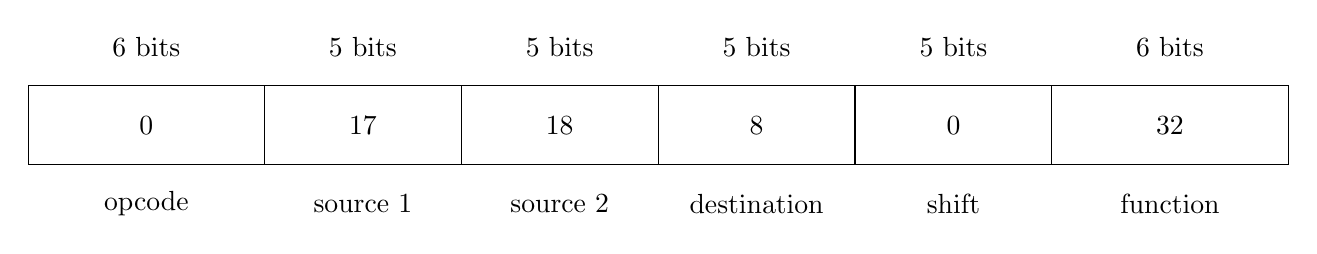
\begin{tikzpicture}
                    \draw
                    (0, 0) -- (16, 0) -- (16, -1) -- (0, -1) -- cycle;

                    \draw
                    (3, 0) -- (3, -1)
                    (5.5, 0) -- (5.5, -1)
                    (8, 0) -- (8, -1)
                    (10.5, 0) -- (10.5, -1)
                    (13, 0) -- (13, -1);

                    \node[] () at (1.5, -0.5) {0};
                    \node[] () at (4.25, -0.5) {17};
                    \node[] () at (6.75, -0.5) {18};
                    \node[] () at (9.25, -0.5) {8};
                    \node[] () at (11.75, -0.5) {0};
                    \node[] () at (14.5, -0.5) {32};

                    \node[] () at (1.5, 0.5) {6 bits};
                    \node[] () at (4.25, 0.5) {5 bits};
                    \node[] () at (6.75, 0.5) {5 bits};
                    \node[] () at (9.25, 0.5) {5 bits};
                    \node[] () at (11.75, 0.5) {5 bits};
                    \node[] () at (14.5, 0.5) {6 bits};

                    \node[] () at (1.5, -1.5) {opcode};
                    \node[] () at (4.25, -1.5) {source 1};
                    \node[] () at (6.75, -1.5) {source 2};
                    \node[] () at (9.25, -1.5) {destination};
                    \node[] () at (11.75, -1.5) {shift};
                    \node[] () at (14.5, -1.5) {function};
                \end{tikzpicture}
            \end{center}
            I-type instructions are used for memory access, conditional branching, or arithmetic with constants. An example of doing addition with constants is \texttt{addi \$1, \$2, 100}, which does reg1 = reg2 + 100. The example displayed below is \texttt{lw \$8, Astart(\$19)}, which does reg8 = M[Astart + reg19].
            \begin{center}
                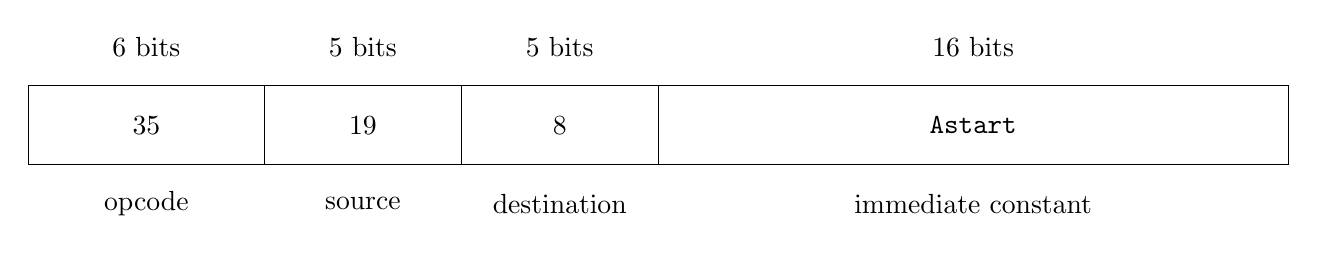
\begin{tikzpicture}
                    \draw
                    (0, 0) -- (16, 0) -- (16, -1) -- (0, -1) -- cycle;

                    \draw
                    (3, 0) -- (3, -1)
                    (5.5, 0) -- (5.5, -1)
                    (8, 0) -- (8, -1);

                    \node[] () at (1.5, -0.5) {35};
                    \node[] () at (4.25, -0.5) {19};
                    \node[] () at (6.75, -0.5) {8};
                    \node[] () at (12, -0.5) {\texttt{Astart}};

                    \node[] () at (1.5, 0.5) {6 bits};
                    \node[] () at (4.25, 0.5) {5 bits};
                    \node[] () at (6.75, 0.5) {5 bits};
                    \node[] () at (12, 0.5) {16 bits};

                    \node[] () at (1.5, -1.5) {opcode};
                    \node[] () at (4.25, -1.5) {source};
                    \node[] () at (6.75, -1.5) {destination};
                    \node[] () at (12, -1.5) {immediate constant};
                \end{tikzpicture}
            \end{center}
            Finally J-type instructions are jump to instructions in memory, for example, \texttt{j 1236} would be an unconditional jump to the instruction at address 1236. An unconditional jump has the following format;
            \begin{center}
                \begin{tikzpicture}
                    \draw
                    (0, 0) -- (16, 0) -- (16, -1) -- (0, -1) -- cycle;

                    \draw
                    (3, 0) -- (3, -1);

                    \node[] () at (1.5, -0.5) {2};
                    \node[] () at (9.5, -0.5) {1236};

                    \node[] () at (1.5, 0.5) {6 bits};
                    \node[] () at (9.5, 0.5) {26 bits};

                    \node[] () at (1.5, -1.5) {opcode};
                    \node[] () at (9.5, -1.5) {memory location};
                \end{tikzpicture}
            \end{center}
            However, we can also have jump instructions, which are I-type, or R-type, for example \texttt{bne \$19, \$20, Label} is an I-type instruction, where the program jumps to \texttt{Label} if registers 19, and 20 aren't equal. An R-type example would be \texttt{jr \$ra}, where it jumps to the address in register ra.

            Consider the following program, and its equivalent in machine code, the registers are labeled in alphabetical order (reg16 = f, reg20 = j, etc);
            \begin{lstlisting}
                if (i == j) {
                  f = g + h;
                } else {
                  f = g - h;
                }

                      bne $\dollar$19, $\dollar$20, Else # if i $\neq$ j goto Else
                      add $\dollar$16, $\dollar$17, $\dollar$18     # f = g + h
                      j   Exit           # goto Exit
                Else: sub $\dollar$16, $\dollar$17, $\dollar$18     # f = g - h
                Exit:
            \end{lstlisting}
            Since we only have two types of conditional branches, \texttt{bne}, and \texttt{beq}, we need \texttt{slt}, which does the following - \texttt{slt \$1, \$16, \$17}, if reg16 $<$ reg17, then it sets reg1 to 1, otherwise it's set to 0. Then, we can use \texttt{bne}, with \texttt{\$0}, since reg0 is always set to logic 0.
        \subsection*{Lecture 2 \hfill P\&H 28-53}
            One of the questions raised in this lecture is the following; "Is a 20\% cheaper processor, with the same performance good enough?". While this may seem straightforward, from a consumer's perspective, it's important to note that a consumer has instant gratification from buying a product, but developing one would take time. In this time, competitors are also trying to improve on their product, and as such you can't just know the price, and performance of a competitor's product \textbf{now}, but you also need to predict the improvement.
            \medskip

            CPI is the \textbf{average} number of clock cycles required per instruction. Note that it's the average, because some instructions may take more cycles to complete. For a given program $P$, we can get the number of cycles required for $P$ by doing the number of instructions in $P$, multiplied by the CPI. The execution time for $P$ is the number of cycles in $P$, multiplied by the clock cycle time (which is $\frac{1}{\text{clock speed}}$). Assuming that for a set of programs $P_1$, ..., $P_n$, the workload is equal, we can calculate the average execution time for the set by taking the mean of the execution times.
            \subsubsection*{Example}
                Consider two machines, $M_1$, and $M_2$, which implement the same instruction set that has 2 classes of instructions; $A$, and $B$. The CPI for $M_1$ on class $A$ is $A_1$, $B$, is $B_1$, and the same for $M_2$. The clock speed of $M_1$ is $C_1$ MHz, and similar for $M_2$. If we were to compare their peak and average performance of $N$ instructions, half of which are of class $A$, and the other half of class $B$, we'd need to find the ratio of execution times.
                \medskip

                In order to find the peak performance of $N$ instructions for $M_1$ (let it be $P_{P1}$), we take the clock cycle time (which is $\frac{1}{C_1}$, multiply it by the number of instructions $N$, miltiply it by the \textbf{minimum} CPI for $M_1$ (which would be min($A_1$, $B_1$)), we'd get $\frac{N(\text{min}(A_1, B_1))}{C_1}$. To compare the two, we take $\frac{P_{P1}}{P_{P2}} = \frac{\text{min}(A_1, B_1) \cdot C_2}{\text{min}(A_2, B_2) \cdot C_1}$.
                \medskip

                We do a similar process for finding the average performance, let it be $P_{A1}$, but instead of multiplying it by the minimum CPI, we take the average, hence we multiply by $\frac{A_1 + B1}{2}$. To compare the two, we take $\frac{P_{A1}}{P_{A2}} = \frac{(A_1 + B_1) \cdot C_2}{(A_2 + B_2) \cdot C_1}$.
                \medskip

                Our goal is to minimize the execution time, which is to minimise $\text{instruction count} \times \text{CPI} \times \text{cycle time}$. Consider this example, comparing SUN 68000, and their newer SUN RISC. In the RISC device, there are 25\% more instructions, and the cycle time is 50\% longer. However, the CPI is much lower, as the instructions are simpler, thus requiring less cycles. The price has increased, but the performance has doubled.
                \begin{center}
                    \begin{tabular}{l|l|l}
                        & SUN 68000 & SUN RISC \\
                        \hline
                        Instruction Count Ratio & 1.0 & 1.25 \\
                        Cycle time & 40ns & 60ns \\
                        CPI & 5.0 - 7.0 & 1.3 - 1.7 \\
                        Execution Time Ratio & 2 & 1 \\
                        Price Ratio & 1 & 1.1 - 1.2
                    \end{tabular}
                \end{center}
                The processor time is measured by the seconds per program, which is calculated as follows; $\frac{\text{time}}{\text{program}} = \frac{\text{instructions}}{\text{program}} \cdot \frac{\text{cycles}}{\text{instruction}} \cdot \frac{\text{time}}{\text{cycle}}$.
            \subsubsection*{RISC}
                Regarding the principles of RISC instruction set design, the common cases should be optimised, thus reducing the CPI. A small number of general purpose registers (32 in MIPS), simplifies things, and allows the design to be more adaptable to new technologies. The smaller chip size allows for a higher yield, thus reducing the cost of production. On the other hand, the lower number of instructions increases the code size, and smarter compilers are needed, since the instructions are further away from the software level than with a CISC instruction set.
            \subsubsection*{Performance Trends}
                In 2004, the trend in power usage hit a peak, due to heat not being able to be removed from the chip at a reasonable rate. The voltage also cannot be reduced further, which is why the trends seemed to have become flat. $P = C \cdot V^2 \cdot F$, where $P$ is power, $C$ is capacitive load, $V$ is voltage, and $F$ is frequency.
                \medskip

                Other than just increasing clock speed, performance can be increased in other ways; including faster local storage, concurrent execution, and newer technologies. Implementning on-chip caches allows for faster execution due to the faster memory closer to the chip, which would be a significant improvement compared to fetching from RAM. Concurrent execution can be achieved by multiple function units (super scalar), a pipeline execution, or multiple instruction streams (multi-threading). Newer technologies, such as GPUs can also be used for specialised loads.
            \subsubsection*{Benchmarking}
                There are a number of ways of benchmarking, each with their benefits, and drawbacks as follows;
                \begin{center}
                    \begin{tabular}{l|l|l}
                        method & pros & cons \\
                        \hline
                        actual target workload & representative & very specific, not portable \\
                        & & difficult to measure \\
                        & & hard to identify problems \\
                        \hline
                        full benchmarks & portable & less representative \\
                        & widespread usage & \\
                        \hline
                        kernel benchmarks & easy to use & peak is not representative \\
                        & used early in design cycle & \\
                        & identify peak performance &
                    \end{tabular}
                \end{center}
        \subsection*{Lecture 3}
            Considering the software side of parallelism; we have parallel requests, parallel threads, parallel instructions, and parallel data. Parallel threads schedule tasks; for example if you have an instruction that takes longer to process since it has to read from main memory, or wait for another resource, another task can be scheduled to run during this time. Since a processor core has multiple functional units, instructions can be arranged in a pipeline, where different stages are processed at the same time. Finally, data can be parallelised, as each item of data can contain multiple chunks of data, each of which can be operated on separately.
            \medskip

            In MIPS, we have 3 different types of addressing;
            \begin{itemize}
                \itemsep0em
                \item register addressing \hfill accessing the data in registers
                \item immediate addressing \hfill data is contained within the instruction (I-type)
                \item base addressing \hfill accessing data in memory with load/store instructions
                \item PC-relative addressing \hfill replaces the register with the program counter (in the I-type load)
            \end{itemize}
            We can classify architectures by how they address temporary storage. Here we cover three main types - all of which are operating on the same code; which is \texttt{C = A + B};
            \begin{itemize}
                \itemsep0em
                \item stack \hfill operands are implicitly specified at the top of the stack
                    \subitem \texttt{push A; push B; add; pop C}
                    \subitem this adds the top pair of items on the stack
                    \subitem pros: it has a simple evaluation model, and the code is dense
                    \subitem cons: this model is less flexible, has no random access, and is slow if the stack is in memory
                \item accumulator \hfill one operand in the accumulator
                    \subitem \texttt{load A; add B; store C}
                    \subitem this adds the accumulator, and the data in memory
                    \subitem pros: there is minimal internal storage, and has short instructions
                    \subitem cons: there is frequent memory access, therefore it is slower
                \item register \hfill we explicitly state the operands
                    \subitem \texttt{load R1 A; add R2, R1, B; store C, R2}
                    \subitem this simply adds two registers
                    \subitem pros: this is the general model for code generation, and has faster register access
                    \subitem cons: this requires you to name all the operands, and also has longer instructions
            \end{itemize}
            Most modern architectures are register based, as it's still faster, as there is less memory traffic, as well as the code being denser. At the start, the first computers used single accumulators, as memory was still expensive, and therefore registers had to be used sparingly.
            \subsubsection*{Amdahl's Law}
                When some instructions are used frequently, and are normally expensive to compute, there are three possible approaches (for example, repeatedly calculating $x^2 + y^2$);
                \begin{enumerate}[1.]
                    \itemsep0em
                    \item add instruciton, accumulator, or load-store
                    \item add, and square instructions, accumulator, or load-store
                    \item custom sumsq instruction, with a dedicated circuit
                \end{enumerate}
                However, this is not always beneficial (or worth the additional cost, and time). For example, consider a program that takes $T_\text{old}$ time to run, and a fraction of the code $\alpha$ can be sped up $\beta$ times. Now, we can calculate the new runtime of the code as $T_\text{new} = \alpha \frac{T_\text{old}}{\beta} + (1 - \alpha)T_\text{old}$. Let's have an example, wehre 90\% of the code can be sped up 100 times, such that $\alpha = 0.9$, and $\beta = 100$. By running this calculation, we can say that $T_\text{old} \approx 9.17 \cdot T_\text{new}$ - the code is less than 10 times faster.
        \subsection*{Lecture 4}
            There are two ways of representing negative numbers in binary, two's complement, and sign-and-magnitude. When we use sign-and-magnitude, it may be more intuitive for us, but for a computer to do addition on it may be problematic as we can easily lose (or gain) the sign bit. On the other hand, two's complement is more complex, but allows for easier operations. For example, you can repeat the most significant bit (e.g. $\texttt{10}_\text{2C} = \texttt{111110}_\text{2C} = -2_\text{Dec}$)
            \medskip

            The layout of a MIPS ALU is similar to the basic one covered in \textbf{CO112}, as in, it has separate units for bit-wise AND, bit-wise OR, addition, etc. and also does the all the operations, then selects one based on the input. Similarly, it also uses the same slash notation to denote $n$ lines being connected. On the gate level, it's important to remember the following;
            \begin{center}
                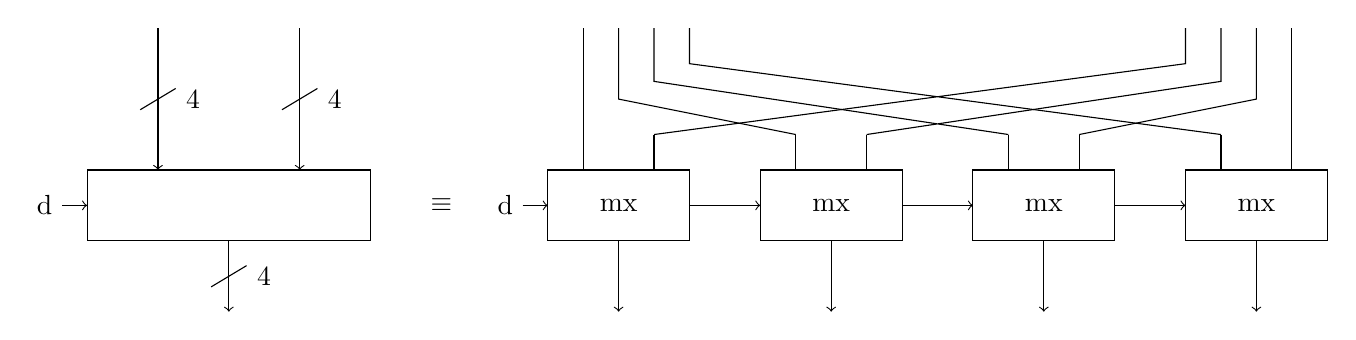
\begin{tikzpicture}[x=0.9cm, y=0.9cm]
                    \node[] (d) at (-0.6, -0.5) {d};
                    \draw
                    (0, 0) -- (4, 0) -- (4, -1) -- (0, -1) -- cycle
                    (1, 2) edge[->] (1, 0)
                    (3, 2) edge[->] (3, 0)
                    (2, -1) edge[->] (2, -2)
                    (d) edge[->] (0, -0.5);

                    \node[] (i1) at (1, 1) {};
                    \node[] (i2) at (3, 1) {};
                    \node[] (o) at (2, -1.5) {};

                    \draw
                    ($(i1) + (-0.25, -0.15)$) edge[right] node{\ \ 4} ($(i1) + (0.25, 0.15)$)
                    ($(i2) + (-0.25, -0.15)$) edge[right] node{\ \ 4} ($(i2) + (0.25, 0.15)$)
                    ($(o) + (-0.25, -0.15)$) edge[right] node{\ \ 4} ($(o) + (0.25, 0.15)$);

                    \node[] (d2) at (5.9, -0.5) {d};
                    \foreach \x in {0,...,3} {
                        \draw
                        (6.5 + 3*\x, 0) -- (8.5 + 3*\x, 0) -- (8.5 + 3*\x, -1) -- (6.5 + 3*\x, -1) -- cycle
                        (7.5 + 3*\x, -1) edge[->] (7.5 + 3*\x, -2)
                        (7 + 3*\x, 0) -- (7 + 3*\x, 0.5)
                        (8 + 3*\x, 0) -- (8 + 3*\x, 0.5);

                        \node[] () at (7.5 + 3*\x, -0.5) {mx};

                        \draw
                        (7 + 0.5*\x, 2) -- (7 + 0.5*\x, 0.75 + 0.25*\x) -- (7 + 3*\x, 0.5)
                        (17 - 0.5*\x, 2) -- (17 - 0.5*\x, 0.75 + 0.25*\x) -- (17 - 3*\x, 0.5);
                    }

                    \draw
                    (d2) edge[->] (6.5, -0.5)
                    (8.5, -0.5) edge[->] (9.5, -0.5)
                    (11.5, -0.5) edge[->] (12.5, -0.5)
                    (14.5, -0.5) edge[->] (15.5, -0.5);

                    \node[] () at (5, -0.5) {$\equiv$};
                \end{tikzpicture}
            \end{center}
            A similar diagram can also be used for the ripple carry adder, which joins $n$ full adders, to create an $n$-bit ripple adder.
            \begin{center}
                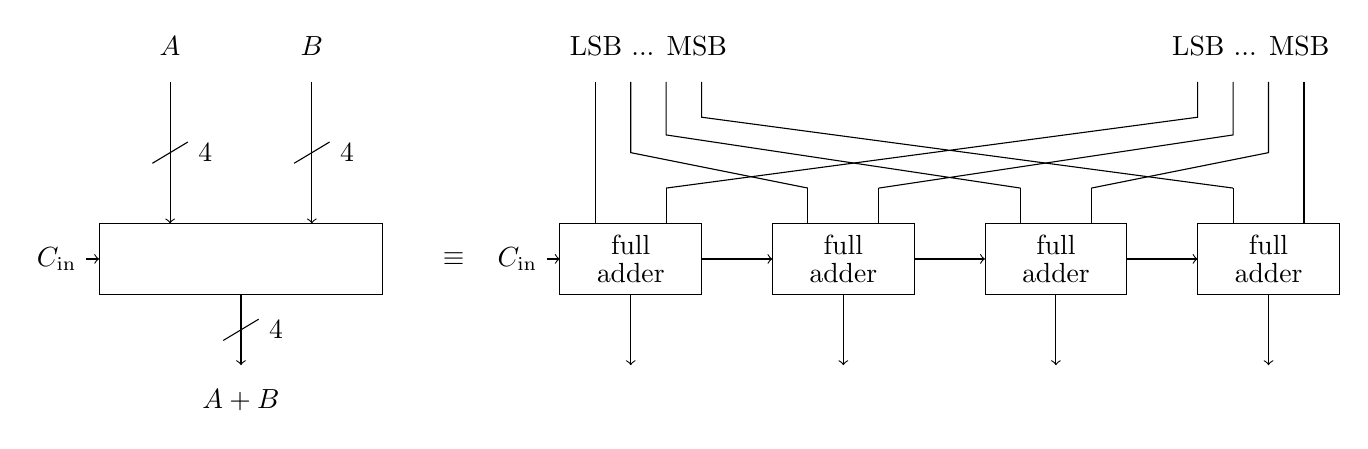
\begin{tikzpicture}[x=0.9cm, y=0.9cm]
                    \node[] (d) at (-0.6, -0.5) {$C_\text{in}$};
                    \draw
                    (0, 0) -- (4, 0) -- (4, -1) -- (0, -1) -- cycle
                    (1, 2) edge[->] (1, 0)
                    (3, 2) edge[->] (3, 0)
                    (2, -1) edge[->] (2, -2)
                    (d) edge[->] (0, -0.5);

                    \node[] (i1) at (1, 1) {};
                    \node[] (i2) at (3, 1) {};
                    \node[] (o) at (2, -1.5) {};

                    \draw
                    ($(i1) + (-0.25, -0.15)$) edge[right] node{\ \ 4} ($(i1) + (0.25, 0.15)$)
                    ($(i2) + (-0.25, -0.15)$) edge[right] node{\ \ 4} ($(i2) + (0.25, 0.15)$)
                    ($(o) + (-0.25, -0.15)$) edge[right] node{\ \ 4} ($(o) + (0.25, 0.15)$);

                    \node[] (d2) at (5.9, -0.5) {$C_\text{in}$};
                    \foreach \x in {0,...,3} {
                        \draw
                        (6.5 + 3*\x, 0) -- (8.5 + 3*\x, 0) -- (8.5 + 3*\x, -1) -- (6.5 + 3*\x, -1) -- cycle
                        (7.5 + 3*\x, -1) edge[->] (7.5 + 3*\x, -2)
                        (7 + 3*\x, 0) -- (7 + 3*\x, 0.5)
                        (8 + 3*\x, 0) -- (8 + 3*\x, 0.5);

                        \node[] () at (7.5 + 3*\x, -0.5) {\shortstack{full\\adder}};

                        \draw
                        (7 + 0.5*\x, 2) -- (7 + 0.5*\x, 0.75 + 0.25*\x) -- (7 + 3*\x, 0.5)
                        (17 - 0.5*\x, 2) -- (17 - 0.5*\x, 0.75 + 0.25*\x) -- (17 - 3*\x, 0.5);
                    }

                    \node[] () at (7.75, 2.5) {LSB ... MSB};
                    \node[] () at (16.25, 2.5) {LSB ... MSB};
                    \node[] () at (1, 2.5) {$A$};
                    \node[] () at (3, 2.5) {$B$};
                    \node[] () at (2, -2.5) {$A+B$};
                    \draw
                    (d2) edge[->] (6.5, -0.5)
                    (8.5, -0.5) edge[->] (9.5, -0.5)
                    (11.5, -0.5) edge[->] (12.5, -0.5)
                    (14.5, -0.5) edge[->] (15.5, -0.5);

                    \node[] () at (5, -0.5) {$\equiv$};
                \end{tikzpicture}
            \end{center}
            With this full adder, we are able to use this as as subtractor. For example, when working with $A - B$; take the ones complement of $B$ (which is inverting $B$ bitwise), and add it to $A$, and setting $C_\text{in}$ to 1. Bitwise inversion is done with an XOR, when the otger input is 1. Other important circuits found in our ALU, are the AOR (which is shown below);
            \begin{center}
                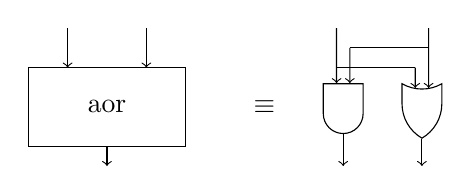
\begin{tikzpicture}
                    \node[] () at (1, 0) {aor};
                    \node[] () at (3, 0) {$\equiv$};

                    \draw
                    (0, 0.5) -- (2, 0.5) -- (2, -0.5) -- (0, -0.5) -- cycle
                    (0.5, 1) edge[->] (0.5, 0.5)
                    (1.5, 1) edge[->] (1.5, 0.5)
                    (1, -0.5) edge[->] (1, -0.75);

                    \node[and gate US, draw, logic gate inputs=nn, rotate=-90] (and) at (4, 0) {};
                    \node[or gate US, draw, logic gate inputs=nn, rotate=-90] (or) at (5, 0) {};

                    \draw
                    (4 - 0.085, 1) edge[->] (and.input 2)
                    (5 + 0.085, 1) edge[->] (or.input 1)
                    (4 - 0.085, 0.5) -- (5 - 0.085, 0.5) edge[->] (or.input 2)
                    (5 + 0.085, 0.75) -- (4+ 0.085, 0.75) edge[->] (and.input 1)
                    (and.output) edge[->] (4, -0.75)
                    (or.output) edge[->] (5, -0.75);
                \end{tikzpicture}
            \end{center}
            This can then be combined with a single full adder block, to create AFA;
            \begin{center}
                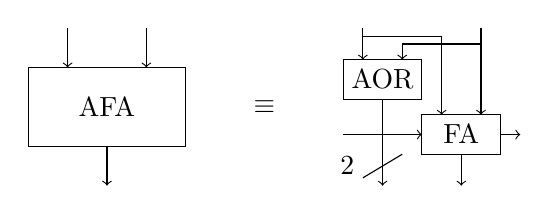
\begin{tikzpicture}
                    \node[] () at (1, 0) {AFA};
                    \node[] () at (3, 0) {$\equiv$};

                    \draw
                    (0, 0.5) -- (2, 0.5) -- (2, -0.5) -- (0, -0.5) -- cycle
                    (0.5, 1) edge[->] (0.5, 0.5)
                    (1.5, 1) edge[->] (1.5, 0.5)
                    (1, -0.5) edge[->] (1, -1);

                    \node[] () at (4.5, 0.35) {AOR};
                    \node[] () at (5.5, -0.35) {FA};
                    \node[] (o) at (4.5, -0.75) {};

                    \draw
                    (4, 0.6) -- (5, 0.6) -- (5, 0.1) -- (4, 0.1) -- cycle
                    (5, -0.1) -- (6, -0.1) -- (6, -0.6) -- (5, -0.6) -- cycle
                    (4.25, 1) edge[->] (4.25, 0.6)
                    (5.75, 1) edge[->] (5.75, -0.1)
                    (4.25, 0.9) -- (5.25, 0.9) edge[->] (5.25, -0.1)
                    (5.75, 0.8) -- (4.75, 0.8) edge[->] (4.75, 0.6)
                    (4.5, 0.1) edge[->] (4.5, -1)
                    (5.5, -0.6) edge[->] (5.5, -1)
                    (4, -0.35) edge[->] (5, -0.35)
                    (6, -0.35) edge[->] (6.25, -0.35)
                    ($(o) + (-0.25, -0.15)$) edge[left] node{2\ \ \ } ($(o) + (0.25, 0.15)$);
                \end{tikzpicture}
            \end{center}
            With these components, we can build our first ALU block;
            \begin{center}
                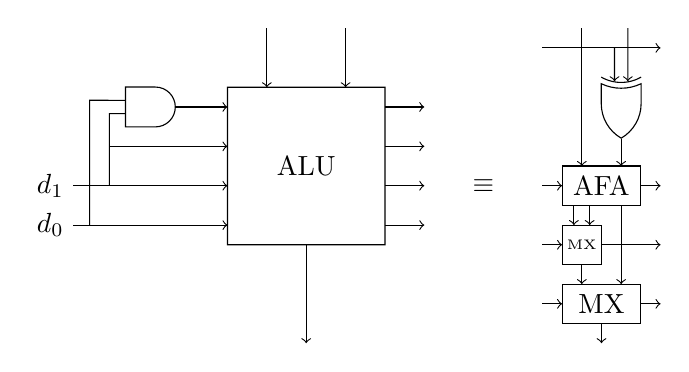
\begin{tikzpicture}
                    \node[and gate US, draw, logic gate inputs=nn] (and) at (0, 0) {};
                    \node[] () at (2, -0.75) {ALU};
                    \node[] (d0) at (-1.25, -1.5) {$d_0$};
                    \node[] (d1) at (-1.25, -1) {$d_1$};
                    \draw
                    (1, 0.25) -- (3, 0.25) -- (3, -1.75) -- (1, -1.75) -- cycle
                    (and.output) edge[->] (1, 0)
                    (-0.5, -0.5) edge[->] (1, -0.5)
                    (d1) edge[->] (1, -1)
                    (d0) edge[->] (1, -1.5)
                    (-0.75, -1.5) -- (-0.75, 0.085) -- (and.input 1)
                    (-0.5, -1) -- (-0.5, -0.085) -- (and.input 2)
                    (1.5, 1) edge[->] (1.5, 0.25)
                    (2.5, 1) edge[->] (2.5, 0.25)
                    (2, -1.75) edge[->] (2, -3)
                    \foreach \x in {0,...,3} {
                        (3, -1.5 + 0.5*\x) edge[->] (3.5, -1.5 + 0.5*\x)
                    };

                    \node[] () at (5.75, -1) {AFA};
                    \node[] () at (5.5, -1.75) {\tiny MX};
                    \node[] () at (5.75, -2.5) {MX};
                    \node[xor gate US, draw, logic gate inputs=nn, rotate=-90] (xor) at (6, 0) {};
                    \node[] () at (4.25, -1) {$\equiv$};
                    \draw
                    (5, 0.75) edge[->] (6.5, 0.75)
                    (6 - 0.085, 0.75) edge[->] (xor.input 2)
                    (6 + 0.085, 1) edge[->] (xor.input 1)
                    (5.25, -0.75) -- (6.25, -0.75) -- (6.25, -1.25) -- (5.25, -1.25) -- cycle
                    (5.25, -1.5) -- (5.75, -1.5) -- (5.75, -2) -- (5.25, -2) -- cycle
                    (5.25, -2.25) -- (6.25, -2.25) -- (6.25, -2.75) -- (5.25, -2.75) -- cycle
                    (5, -1) edge[->] (5.25, -1)
                    (5, -1.75) edge[->] (5.25, -1.75)
                    (5, -2.5) edge[->] (5.25, -2.5)
                    (6.25, -1) edge[->] (6.5, -1)
                    (5.75, -1.75) edge[->] (6.5, -1.75)
                    (6.25, -2.5) edge[->] (6.5, -2.5)
                    (xor.output) edge[->] (6, -0.75)
                    (5.5, 1) edge[->] (5.5, -0.75)
                    (5.4, -1.25) edge[->] (5.4, -1.5)
                    (5.6, -1.25) edge[->] (5.6, -1.5)
                    (5.5, -2) edge[->] (5.5, -2.25)
                    (6, -1.25) edge[->] (6, -2.25)
                    (5.75, -2.75) edge[->] (5.75, -3);
                \end{tikzpicture}
            \end{center}
            This design for the ALU has the functions $d_0d_1$, where 00 is AND, 01 is OR, 10 is addition, and 11 is subtraction. Remember that the carry is only set to 1 at the start when we're doing subtraction. The top line is also set to 1 when we're doing subtraction.
            \medskip

            The carry path is often the slowest line, as it needs to go through many gates of logic, which limits the clock rate, since clock rate $\approx \frac{1}{\text{delay of slowest path}}$, given we have an edge-triggered design, and a few other factors (from P\&H Appendix B. 11)
        \subsection*{Lecture 5 \hfill P\&H 183-196}
            \subsubsection*{Multiplication Algorithm}
                Consider the example $2 \cdot 11 = 22$, we have the multiplicand times the multiplier = product. However, to do this bitwise, we have to do the following (let $c \leftarrow n$ mean $c$ shifted $n$ bits to the left, and $b_i$ mean the $i^\text{th}$ bit of $b$);
                \begin{center}
                    \begin{tabular}{cccccccccl}
                        & & & & & 0 & 0 & 1 & 0 & multiplicand ($c$) \\
                        $\times$ & & & & & 1 & 0 & 1 & 1 & multiplier ($p$) \\
                        \hline
                        & & & & & 0 & 0 & 1 & 0 & $(c \leftarrow 0) \cdot p_0$ \\
                        & & & & 0 & 0 & 1 & 0 & & $(c \leftarrow 1) \cdot p_1$ \\
                        & & & 0 & 0 & 0 & 0 & & & $(c \leftarrow 2) \cdot p_2$ \\
                        + & & 0 & 0 & 1 & 0 & & & & $(c \leftarrow 3) \cdot p_3$ \\
                        \hline
                        & & 0 & 0 & 1 & 0 & 1 & 1 & 0 &
                    \end{tabular}
                \end{center}
                Note that the third line is all 0s, because $p_2$ is 0, and multiplication is just AND. The idea is that the product is the miltiplicand shifted succesively by 1 bit relative to the multiplier; CSAA - conditional shift and add. We only really need to shift when the bit isn't 0.
            \subsubsection*{Another Multiplication Algorithm}
                However, there are other options for multiplication algorithms, which can save silicon space; we can use a 32-bit ALU, and a 64-bit register, which stores both the product, and the multiplier initially.
                \begin{center}
                    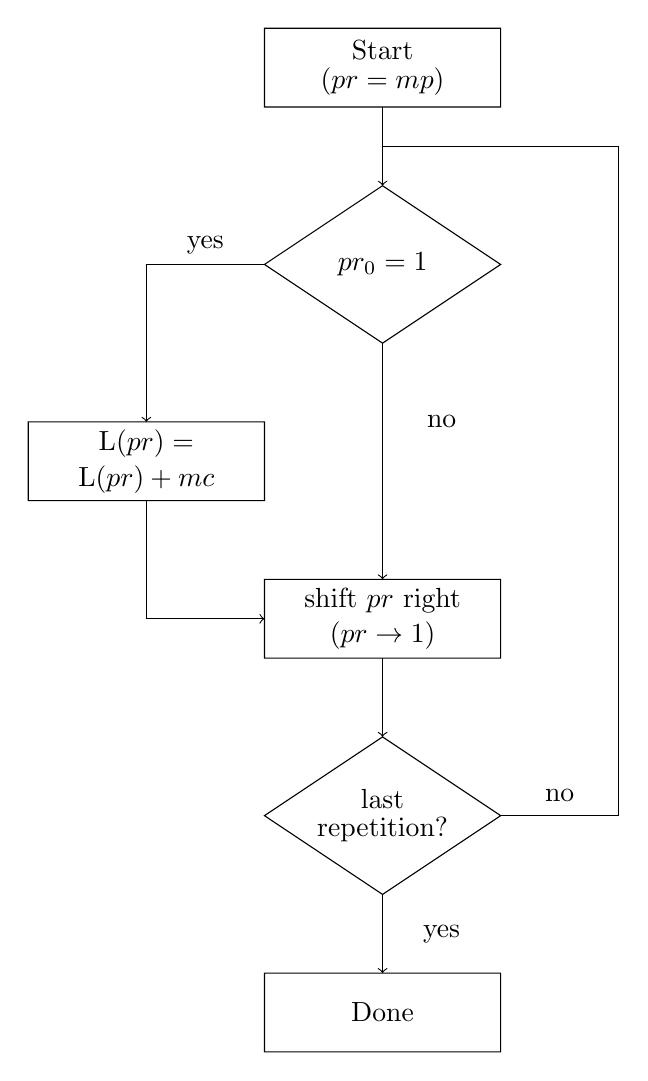
\begin{tikzpicture}[x=1.5cm, y=1cm]
                        \draw
                        (-1, 0) -- (1, 0) -- (1, -1) -- (-1, -1) -- cycle
                        (0, -2) -- (1, -3) -- (0, -4) -- (-1, -3) -- cycle
                        (-3, -5) -- (-1, -5) -- (-1, -6) -- (-3, -6) -- cycle
                        (-1, -7) -- (1, -7) -- (1, -8) -- (-1, -8) -- cycle
                        (0, -9) -- (1, -10) -- (0, -11) -- (-1, -10) -- cycle
                        (-1, -12) -- (1, -12) -- (1, -13) -- (-1, -13) -- cycle;

                        \draw
                        (0, -1) edge[->] (0, -2)
                        (-1, -3) -- (-2, -3) edge[->] (-2, -5)
                        (-2, -6) -- (-2, -7.5) edge[->] (-1, -7.5)
                        (0, -4) edge[->] (0, -7)
                        (0, -8) edge[->] (0, -9)
                        (0, -11) edge[->] (0, -12)
                        (1, -10) -- (2, -10) -- (2, -1.5) -- (0, -1.5);

                        \node[] () at (0, -0.5) {\shortstack{Start \\ $(pr = mp)$}};
                        \node[] () at (0, -3) {$pr_0 = 1$};
                        \node[] () at (-1.5, -2.75) {yes};
                        \node[] () at (0.5, -5) {no};
                        \node[] () at (-2, -5.5) {\shortstack{$\text{L}(pr) =$ \\ $\text{L}(pr) + mc$}};
                        \node[] () at (0, -7.5) {\shortstack{shift $pr$ right \\ $(pr \rightarrow 1)$}};
                        \node[] () at (0, -10) {\shortstack{last \\ repetition?}};
                        \node[] () at (0.5, -11.5) {yes};
                        \node[] () at (1.5, -9.75) {no};
                        \node[] () at (0, -12.5) {Done};
                    \end{tikzpicture}
                \end{center}
            \subsubsection*{Booth's Algorithm}
                When we have a string of repeated 1s, we can change $n$ additions into 1 addition, and 1 subtraction. As we're summing a geometric series, when we do repeated additions, such that $m + 2m + 2^2m + ... + 2^{k-1}m = -m + 2^km$. This is much easier to compute, as all we have to do is to do an arithmetic shift on $m$, and a subtraction. However, instead of checking only the LSB ($pr_0$), we also check the previous LSB, let it be $pr_{-1}$. We have the following cases, written $pr_0pr_{-1}$; 00 or 11 - we're in the middle of a string of 0s (or 1s, respectively), no action is needed, 01 - we're at the end of a string of 1s, $pr = pr + mc$ (where $mc$ is the shifted multiplicand), and 10 - we're at the start of a string of 1s, $pr = pr - mc$. Note that in my version of the slides (2018 - 2019 academic year), there is a typo on slide 15. The "corrected" version is below (this is working on $\texttt{0010}_2 \times \texttt{0110}_2$), and $mc$ is \texttt{0010}. Also note that $\text(pr)$ means the left half of the product register;
                \begin{center}
                    \begin{tabular}{c|lr|lr}
                        iteration & \multicolumn{2}{c|}{original} & \multicolumn{2}{c}{Booth's} \\
                        & step & product & step & product \\
                        \hline
                        0 & initial values & 0000 011\textbf{0} & initial values & 0000 011\textbf{0} \textbf{0} \\
                        \hline
                        1 & 1a: 0 - no operation & 0000 0110 & 1a: 00 - no operation & 0000 0110 0 \\
                        & 2: product shift right & 0000 001\textbf{1} & 2: product shift right & 0000 001\textbf{1} \textbf{0} \\
                        \hline
                        2 & 1b: 1 - $\text{L}(pr) = \text{L}(pr) + mc$ & 0010 0011 & 1c: 10 - $\text{L}(pr) = \text{L}(pr) - mc$ & 1110 0011 0 \\
                        & 2: product shift right & 0001 000\textbf{1} & 2: product shift right & 1111 000\textbf{1} \textbf{1} \\
                        \hline
                        3 & 1b: 1 - $\text{L}(pr) = \text{L}(pr) + mc$ & 0011 0001 & 1d: 11 - no operation & 1111 0001 1 \\
                        & 1: product shift right & 0001 100\textbf{0} & 2: product shift right & 1111 100\textbf{0} \textbf{1} \\
                        \hline
                        4 & 1a: 0 - no operation & 0001 1000 & 1b: 01 - $\text{L}(pr) = \text{L}(pr) + mc$ & 0001 1000 1 \\
                        & 1: product shift right & 0000 1100 & 2: product shift right & 0000 1100 0 \\
                    \end{tabular}
                \end{center}
            \subsubsection*{Division}
                This algorithm was invented by Briggs; dividend = quotient $\times$ divisor + remainder. We can work through an example of the first algorithm as follows; case 2b is when $rem < 0$, and 2a is when $rem \geq 0$. Note that SLL means we are doing a logical left shift on the quotient, and SR means we are shifting the divisor to the right. This is working through $\frac{7}{2}$;
                \begin{center}
                    \begin{tabular}{c|l|c|c|c}
                        iteration & step & quotient & divisor & remainder \\
                        \hline
                        0 & initial values & 0000 & 0010 0000 & 0000 0111 \\
                        \hline
                        1 & 1: $rem = rem - div$ & 0000 & 0010 0000 & 1110 0111 \\
                        & 2b: $rem = rem + div$; SLL; $Q_0$ = 0 & 0000 & 0010 0000 & 0000 0111 \\
                        & c: SR & 0000 & 0001 0000 & 0000 0111 \\
                        \hline
                        2 & 1: $rem = rem - div$ & 0000 & 0001 0000 & 1111 0111 \\
                        & 2b: $rem = rem + div$; SLL; $Q_0$ = 0 & 0000 & 0001 0000 & 0000 0111 \\
                        & c: SR & 0000 & 0000 1000 & 0000 0111 \\
                        \hline
                        3 & 1: $rem = rem - div$ & 0000 & 0000 1000 & 1111 1111 \\
                        & 2b: $rem = rem + div$; SLL; $Q_0$ = 0 & 0000 & 0000 1000 & 0000 0111 \\
                        & c: SR & 0000 & 0000 0100 & 0000 0111 \\
                        \hline
                        4 & 1: $rem = rem - div$ & 0000 & 0000 0100 & 0000 0011 \\
                        & 2a: SLL; $Q_0$ = 1 & 0001 & 0000 0100 & 0000 0011 \\
                        & c: SR & 0001 & 0000 0010 & 0000 0011 \\
                        \hline
                        5 & 1: $rem = rem - div$ & 0001 & 0000 0010 & 0000 0001 \\
                        & 2a: SLL; $Q_0$ = 1 & 0011 & 0000 0010 & 0000 0001 \\
                        & c: SR & 0011 & 0000 0001 & 0000 0001
                    \end{tabular}
                \end{center}
                Similar to multiplication, we can refine our implementation of division by replacing the divisor shift to the right, with a remainder shift to the left. By doing this, we can reduce the 64-bit ALU to 32 bits. As we are shifting the remainder to the left, and we're doing the same shift to the quotient, we can combine the registers like before.
        \subsection*{Lecture 6 \hfill P\&H 244-272}
            Seriously, for this lecture, just look at the slides. There's too many diagrams for me to draw in TikZ.
            \medskip

            In general, the control unit is just a combinatorial unit, which takes in the 6 bits from the opcode, and has a 9-bit output, which controls the multiplexers, ALU, and the read / write operations. The initial implementation was having separate datapaths for the different types of instructions; register-based, memory-based, and branch. This can then be combined with multiplexors, which allow the right blocks to be conected, and finally the control unit unifies it by activating relavent parts of the combined datapath, based on the instruciton.
            \medskip

            Note that often the addresses for instructions will increment in 4, since memory is normally byte addressable, and the instructions we are working with are 32-bit. The design in the slides abstract the circuit into a single cycle data path, but it's important to note that it isn't the case, especially due to memory access as that would require more cycles.
        \subsection*{Lecture 7}
            The following accesses are needed in the execution cycle;
            \begin{center}
                \begin{tabular}{c|ccccc}
                    type & instruction fetch & read register & ALU operation & load / store data & write to register \\
                    \hline
                    R-type & $\checkmark$ & $\checkmark$ & $\checkmark$ & & $\checkmark$ \\
                    load & $\checkmark$ & $\checkmark$ & $\checkmark$ & $\checkmark$ & $\checkmark$ \\
                    store & $\checkmark$ & $\checkmark$ & $\checkmark$ & $\checkmark$ & \\
                    branch & $\checkmark$ & $\checkmark$ & $\checkmark$ & & \\
                    jump & $\checkmark$ & & & &
                \end{tabular}
            \end{center}
            From the above, you will notice that some operations take multiple stages to do, such as load taking all 5, and jump taking only 1. Due to the single clock cycle data path design, all of them take one cycle to finish, regardless of the number of steps. As clocks have a fixed tick time, jump will still take the same amount of time as load, even though it's a much faster instruction.
            \subsubsection*{Multi-cycle datapath}
                This comes with multiple advantages; we're likely to have shorter cycles, but will need more of them (for example, R-type instructions would need 4 cycles to complete, and jump would only need 1). We can also combine memory together, such that instruction, and data are stored in the same location. The ALU can also be reused, but we'd also need the IR, which stores the instruction. More registers will be needed to save the state, leading to a more complex control unit.
                \medskip

                In order to build this, we'd need new internal registers; IR, A, B, $\text{ALU}_\text{out}$, MDR.
                \medskip

                For example, when working on the load instruction, which has the effect;
                \smallskip

                Reg[$\underbrace{\text{dest}}_\text{IR$_{20-16}$}$] = M[Reg[$\underbrace{\text{source}}_\text{IR$_{25-21}$}$] + sign-ext($\underbrace{\text{addr}}_\text{IR$_{15-0}$}$)]
                \medskip

                This instruction can be broken down into smaller steps, as follows, which are RTL (Register Transfer Level) descriptions;
                \begin{enumerate}[{cycle} 1:]
                    \itemsep0em
                    \item IR = M[PC], PC = PC + 4
                    \item A = Reg[source]
                    \item ALU$_\text{out}$ = A + sign-ext(addr)
                        \subitem the sign for addr needs to be extended to a 32-bit number, as the ALU is 32-bit
                    \item MDR = M[ALU$_\text{out}$]
                    \item Reg[dest] = MDR
                \end{enumerate}
                We can tabulate all the execution steps as the following;
                \begin{center}
                    \scalebox{0.875}{
                        \begin{tabular}{c|c|c|c|c}
                            Step & R-type & memory-reference & branches & jumps \\
                            \hline
                            Instruction fetch & \multicolumn{4}{c}{IR = M[PC]} \\
                            & \multicolumn{4}{c}{PC = PC + 4} \\
                            & \multicolumn{4}{c}{\textcolor{blue}{$S_0$}} \\
                            \hline
                            Instruction decode & \multicolumn{4}{c}{A = Reg[IR$_\text{25-21}$]} \\
                            or register fetch & \multicolumn{4}{c}{B = Reg[IR$_\text{20-16}$]} \\
                            & \multicolumn{4}{c}{ALU$_\text{out}$ = PC + (sign-extend(IR$_\text{15-0}$) $<<$ 2)} \\
                            & \multicolumn{4}{c}{\textcolor{blue}{$S_1$}} \\
                            \hline
                            Execution, address & ALU$_\text{out}$ = A op B & ALU$_\text{out}$ = A + & if (A == B) then & PC = PC[IR$_\text{31-28}$] \\
                            computation, branch & & sign-extend(IR$_\text{15-0}$) & PC = ALU$_\text{out}$ & $||$ (IR$_\text{25-0}$ $<<$ 2) \\
                            or jump completion & \textcolor{blue}{$S_6$} & \textcolor{blue}{$S_2$} & \textcolor{blue}{$S_8$} & \textcolor{blue}{$S_9$} \\
                            \hline
                            Memory access or & Reg[IR$_\text{15-11}$] & load: MDR = M[ALU$_\text{out}$] \textcolor{blue}{$S_3$} & & \\
                            R-type completion & = ALU$_\text{out}$ \textcolor{blue}{$S_7$} & store: M[ALU$_\text{out}$] = B \textcolor{blue}{$S_5$} & & \\
                            \hline
                            Memory read & & load: Reg[IR$_\text{20-16}$] = MDR & & \\
                            completion & & \textcolor{blue}{$S_4$} & & \\
                            \hline
                        \end{tabular}%sign-extend(IR$_\text{15-0}$)
                    }
                \end{center}
                Once again, just like in \textbf{CO112}, this can be modelled as a state transition diagram, with the input being determined by the control unit.
        \subsection*{Lecture 8 \hfill P\&H C.3-C.6}
            One of the main issues with our representation of the control unit output logic as a direct FSM is the size, which would have be around $2^10 \cdot 20$, which is roughly 20.5Kbits. Another issue is the readability of it all; while it's very sequential (and we can exploit that later), especially without grouping the outputs. Hence if we were to define fields, we can have each one correspond to one, or more, control signal(s) to acheive a task. For example, if we were to define SRC1 as a field, we could say that SRC1 = A means that ALUSrcA = 1. By assigning values to a field, which represents a control signal assignment, we reach a higher level of abstraction (further than listing the indvidual signals in the state diagram). Another example is having ALU$_\text{control}$ be Add, Fn, or Sub, with the codes 00, 10, or 01 respectively. We can tabulate this as such;
            \begin{center}
                \scalebox{0.9}{
                    \begin{tabular}{cllllllll}
                        state & label & ALU control & SRC1 & SRC2 & memory & reg. control & PC write control & sequencing \\
                        \hline
                        0 & Fetch & Add & PC & 4 & ReadPC & & ALU & Seq \\
                        1 & & Add & PC & ExtShft & & Read & & Dispatch 1 \\
                        2 & Mem1 & Add & A & Extend & & & & Dispatch 2 \\
                        3 & LW2 & & & & ReadALU & & & Seq \\
                        4 & & & & & & WriteMDR & & Fetch \\
                        5 & SW2 & & & & WriteALU & & & Fetch \\
                        6 & Rformat1 & Fn & A & B & & & & Seq \\
                        7 & & & & & & WriteALU & & Fetch \\
                        8 & BEQ1 & Sub & A & B & & & ALU outcond & Fetch \\
                        9 & JUMP1 & & A & B & & & Jump addr & Fetch \\
                    \end{tabular}
                }
            \end{center}
            \begin{center}
                \begin{tikzpicture}
                    \draw
                    (-1, -1.5) edge[->] (0, -1.5)
                    (-1, -2.5) edge[->] (0, -2.5)
                    (-1, -3.5) edge[->] (0, -3.5)
                    (2, -2) edge[->] (3, -2)
                    (5, -2) edge[->] (6, -2)
                    (5.5, -2) -- (5.5, 1.5) edge[->] (2, 1.5)
                    (0, 1.5) -- (-3, 1.5) -- (-3, -0.5) edge[->] (0, -0.5)
                    (-4.5, -2) -- (-3.5, -2)
                    (-3.5, -1.5) -- (-3.5, -2.5)
                    (-3.5, -1.5) edge[->] (-3, -1.5)
                    (-3.5, -2.5) edge[->] (-3, -2.5)
                    (9, -1.5) edge[->] (10, -1.5)
                    (9, -2.5) -- (10, -2.5) -- (10, -5) -- (1, -5) edge[->] (1, -4);

                    \node[] (p6) at (-4, -2) {};
                    \node[] (p4) at (5.5, -0.25) {};
                    \node[] (p16) at (9.5, -1.5) {};
                    \node[] (p2) at (9.5, -2.5) {};
                    \node[] () at (-1.25, -3.5) {0};
                    \node[] () at (1, 1.5) {+1};
                    \node[] () at (-2, -1.5) {DR2};
                    \node[] () at (-2, -2.5) {DR1};
                    \node[] () at (-5.3, -2) {opcode};
                    \node[] () at (4, -2) {$\mu$PC};
                    \node[] () at (1, -2) {MX};
                    \node[] () at (7.5, -2) {\shortstack{combinatorial \\ control logic}};

                    \draw
                    (0, 0) -- (2, 0) -- (2, -4) -- (0, -4) -- cycle
                    (3, 0) -- (5, 0) -- (5, -4) -- (3, -4) -- cycle
                    (6, -1) -- (9, -1) -- (9, -3) -- (6, -3) -- cycle
                    (0, 2) -- (2, 2) -- (2, 1) -- (0, 1) -- cycle
                    (-3, -1.1) -- (-1, -1.1) -- (-1, -1.9) -- (-3, -1.9) -- cycle
                    (-3, -2.1) -- (-1, -2.1) -- (-1, -2.9) -- (-3, -2.9) -- cycle
                    ($(p6) + (-0.25, -0.15)$) edge[above] node{6} ($(p6) + (0.25, 0.15)$)
                    ($(p2) + (-0.25, -0.15)$) edge[below] node{2} ($(p2) + (0.25, 0.15)$)
                    ($(p4) + (-0.25, -0.15)$) edge[right] node{\ \ 4} ($(p4) + (0.25, 0.15)$)
                    ($(p16) + (-0.25, -0.15)$) edge[above] node{16} ($(p16) + (0.25, 0.15)$);
                    ;
                \end{tikzpicture}
            \end{center}
            Note that we'll still have to define DR1, and DR2, the dispatch ROMs. However, the total size of this is around 0.8Kbits, compared to the 20.5Kbits we had before. We could also perform vertical encoding on the output logic, which would reduce the control logic signals, but this comes with its own drawbacks. Horizontal microencoding (which is what we have now) exploits parallelism, and has very little control overhead, however it requires a larger ROM. On the other hand, vertical encoding can be slow, due to the decoding delay.
        \subsection*{Lecture 9}
            Note that pipelining is not examined. In order to handle unexpected events, the processor has to implement addtional circuitry. There are two types of unexpected events that can occur, which both have to be handled with extreme urgency;
            \begin{itemize}
                \itemsep0em
                \item interruptions
                    \subitem these are external events that disrupt the execution cycle, such as input or output, like the power button being pressed
                \item exceptions
                    \subitem these are unexpected events from a program, such as an invalid opcode, or integer overflows
            \end{itemize}
            In the event of an emergency, the program has to do the following;
            \begin{enumerate}[1.]
                \itemsep0em
                \item find out the cause
                    \subitem in order to handle the error, the processor will have to find out the reason
                    \subitem this is done by having an additional register, the Cause register, which is also 32 bits
                \item return to normal execution (sometimes)
                    \subitem in order to retain the program execution point, we need to store the restart address in the exception program counter (EPC)
                    \subitem the control is then transferred to the OS by executing instructions run at the exception address, which is a constant wired into the PC multiplexer
            \end{enumerate}
            To implement this, we also need to modify the finite state machines to have additional states for each error (see the lecture slides for the example).
        \subsection*{Interlude and Introduction}
            As the YouTube playlist covers most of the content, I will be using that as the main point of reference, and not Panopto.
            \bigskip

            While we'd rather write Java, or C, because it's more human friendly, hardware requires strings of bytes which are voltage highs, and lows. While machine code was fine at the start, when machines became more complex, and we could no longer keep up. At this point, we were able to use assembly, which would have equivalent instructions in machine code, but were still human readable. After this, we have an even higher level of abstraction, where a single line of a high-level language, like C, or Java, can be compiled into many lines of assembly. The current lifetime of a program is having the user written program in a high level language, compiled to assembly, which is then compiled to machine code, and run on the hardware.
            \medskip

            During the compilation, the compiler can run optimisations on the code, allowing it to be more efficient to some extent, without the programmer having to do so.
        \subsection*{Memory \& Data}
            \subsubsection*{Memory, data, and Addressing}
                Data needs to be moved from memory to registers, in order for the CPU to operate on it (mentioned in the first part of the module). There's also an instruction cache on the CPU that holds recently used instructions, such as loops - all handled by hardware.
                \medskip

                The bandwidth between the memory, and CPU can limit performance (bottleneck). There are two ways to improve performance; either improving the hardware, or by having larger memory in the chip (cache).
                \medskip

                The transition between voltages can limit the speed of our processor, as we don't want values within the intdeterminate range (between 0.5v, and 2.8v - arbitrary).
            \subsubsection*{Bits, Bytes, and Words}
                In binary, a byte is 8 bits. Converting between hexadecimal, binary, and decimal should be trivial. A byte is two hex digits, hex numbers are represented in C, as \texttt{0xFFF3FF1F} etc. Memory is also byte addressable, and normally an OS provides an \textbf{address space} which is private to each process. A program can modify data in its own state, but not others.
                \medskip

                Each machine has a \textbf{word size}, which is the nominal size of integers in a given machine. Older machines ran on 32-bit words, which limited address to 4GB, but that was too small for intensive applications. However, most modern x86 systems are now on 64-bit words, which allows for around 18 exabytes of memory. In order to group words, we address the word by the address of the first byte, for example, the address of the second word in a 64-bit machine would be 0008$_{10}$.
            \subsubsection*{Memory Addresses}
                An address is a location in memory, a pointer is a data object which contains an address. These are the sizes of objects, in bytes;
                \begin{center}
                    \begin{tabular}{ll|rr}
                        Java & C & 32-bit & x86-64 \\
                        \hline
                        boolean & bool & 1 & 1 \\
                        byte & char & 1 & 1 \\
                        char & & 2 & 2 \\
                        short & short int & 2 & 2 \\
                        int & int & 4 & 4 \\
                        float & float & 4 & 4 \\
                        & long int & 4 & 8 \\
                        double & double & 8 & 8 \\
                        long & long long & 8 & 8 \\
                        & long double & 8 & 16 \\
                        (reference) & pointer * & 4 & 8
                    \end{tabular}
                \end{center}
                In big endian notation, the MSB has the lowest address, whereas in little endian, LSB has the lowest address. Little endian is used in x86, which is what we'll be using.
            \subsubsection*{Addressess, and Pointers in C}
                To be completely honest, this isn't all that useful for this module. But it helps build some understanding.
                \begin{lstlisting}
                    int x, y; /* finds two locations in memory to store 2 integers */
                    int *ptr; /* declares a variable ptr, which points to an integer data item */
                    ptr = &x; /* assigns ptr to point to the address of x */
                    y = *ptr + 1; /* same as y = x + 1; */
                \end{lstlisting}
            \subsubsection*{Arrays}
                Arrays are adjacent locations in memory, which store the same type.
                \begin{lstlisting}
                    int big_array[128]; /* allocates 512 adjacent bytes in memory (128 * 4) */
                    int *array_ptr;
                    array_ptr = &big_array[i];
                    array_ptr = &big_array[0] + i*sizeof(big_array[0]); /* same as above line */
                \end{lstlisting}
                C-style strings are represented as an array of bytes, with a null terminator, which is just a byte of 0s. In order to compute the length of this string, we'd count up until we reach the null terminator.
            \subsubsection*{Boolean Algebra, and Bit Manipulation}
                We really could just skip this, since it's fully covered in \textbf{CO112}, and \textbf{CO140}. The same bit vector operations can be done on any integeral data type in C (\texttt{long}, \texttt{int}, \texttt{short}, and \texttt{char}).
                \begin{lstlisting}
                    p && *p++; /* avoids null pointers, as 0 is false */
                    /* short for the below */
                    if (p) {
                      *p++;
                    }
                \end{lstlisting}
                Bit vectors can be used to represent sets, when we have a $w$-bit vector, representing a set $A = \{0, ..., w - 1\}$, such that bit $a_j == 1 \leftrightarrow j \in A$. This way, we can do bitwise operations, such as doing intersection, union, symmetric difference, and complement.
        \subsection*{Numbers}
\end{document}